\documentclass[12pt, a4paper]{article}
\usepackage{amssymb,
			pgfplots,
			mathtools,
			esint,
			amsthm,
			tikz,
			float,
			hyperref,
			paralist,
			multicol,
			fullpage,
			subcaption,
			esint,
			wrapfig,
			enumitem
			}
\usepackage[makeroom]{cancel}
% \usepackage[English]{babel}
\usepackage{fontspec}
\usepackage[parfill]{parskip}

%pgfplots defaults and fillbetween library
\pgfplotsset{tikzDefaults/.style=
				{
				axis lines = middle,		%axis style
				x label style={at={(axis description cs:1.0, 0.5)},anchor=west},
				y label style={at={(axis description cs:0.5, 1.0)},anchor=south},
				axis line style ={<->, color = black},
				legend style = {draw=none},
				legend columns = 2,
				},
			compat=1.8,
			}
\usepgfplotslibrary{fillbetween}

%remove section numbers
\setlength{\columnsep}{0.9cm}
\setcounter{secnumdepth}{1}

%styling for amsthm
\theoremstyle{plain}
\newtheorem{thm}{Theorem} % reset theorem numbering for each chapter
\newtheorem{cor}{Corollary}
\newtheorem{rem}{Remark}
\newtheorem{lemma}{Lemma}

\theoremstyle{definition}
\newtheorem{definition}{Definition} % definition numbers are dependent on theorem numbers
\newtheorem{example}{Example} % same for example numbers

\newcommand{\gives}{\quad\Rightarrow\quad}
\newcommand{\parder}[2]{\frac{\partial {#1}}{\partial {#2}}}
\newcommand{\HRule}{\rule{\linewidth}{0.5mm}} % Defines a new command for the horizontal lines, change thickness here


\begin{document}

	\thispagestyle{empty}
	\begin{center}
		\textsc{\Large Complex Analysis, 10C 2017}\\[0.5cm] % Major heading such as course name
		\textsc{\large }\\[0.5cm] % Minor heading such as course title
		
		%------------------
		%	TITLE SECTION
		%------------------
		\HRule \\[0.4cm]
		{ \huge \bfseries Lecture Notes}\\[0.2cm] % Title of your document
		
		\HRule \\[1.5cm]
		\large Pouya Ashraf\\[3cm]% Your name
		
		\parbox{12cm}{In this document are lecture notes for the course complex analysis, which was given by Jörgen Östensson at Uppsala University in 2017. All figures are drawn with vector graphics directly in \LaTeX, so that you can zoom in if anything is unclear (fantastic, right?).}\\[3cm]


		{\large \today} % Date

		\newpage
		\vspace*{\fill}
			\parbox{12cm}{Du you appreciate that all relevant info for the course is more or less contained in this document so that you (possibly) don't have to boy the course literature? Do you want to increase the quality of my life marginally, as a thank you for the work I put into this? Send any amount of money with swish to \mbox{070-422 40 81}}\\
		\vspace*{\fill}
	\end{center}
	\newpage

	\pagenumbering{Roman}
	\tableofcontents
	\newpage
	
	\pagenumbering{arabic}
	\section{Introduction} % (fold)
	\label{sec:introduction}
		\begin{definition}
			A complex number is a number on the form $x+iy$, where $x,y\in\mathbb{R}$. Two omplex numbers $x_1+iy_1$, $x_2+iy_2$ are said to be equal iff. $x_1=x_2$ and $y_1=y_2$. The number $x$ is called the real part, and the number $y$ is called the imaginary part.

			We write $x=\mathfrak{Re}(x+iy)$, $y=\mathfrak{Im}(x+iy)$. The set of complex numbers is denoted $\mathbb{C}$.

			We define addition and multiplication as follows:
			\begin{align*}
				(x_1+iy_1)+(x_2+iy_2) &= (x_1+x_2) + i(y_1+y_2)\\
				(x_1+iy_1)\cdot(x_2+iy_2) &= (x_1x_2-y_1y_2)+i(x_1y_2+x_2y_1)
			\end{align*}
			complex numbers are often denoted by $z$ or $w$.\\
		\end{definition}

			\begin{minipage}{0.55\textwidth}
				\begin{definition}
					The complex conjugate of $z=x+iy$ is denoted $\overline{z}$ and is defined by $\overline{z}=x-iy$. It holds that
					\begin{align*}
						\overline{z_1+z_2} &= \overline{z_1}+\overline{z_2}\\
						\overline{z_1\cdot z_2} &= \overline{z_1}\cdot\overline{z_2}.
					\end{align*}
					Note also that $\mathfrak{Re}(z)=\dfrac{z+\overline{z}}{2}$, $\mathfrak{Im}=\dfrac{z-\overline{z}}{2i}$.

					It is natural to represent a complex number $z=x+iy$ as a point $(x,y)\in\mathbb{R}^2$. Thus geometric representation is called the complex/Argand plane.
				\end{definition}
			\end{minipage}
			\begin{minipage}{0.45\textwidth}
				\begin{figure}[H]
				 	\flushright
				 	\begin{tikzpicture}[scale=0.9, transform shape]
				 		\begin{axis}
				 			[
							% height = \textwidth,
							% width = \textwidth,
							ymin = -5, ymax = 5,
							xmin = -5, xmax = 5,
							% ytick = \empty,
							% xtick= \empty,
							xlabel = $\mathfrak{Re}$,
							ylabel = $\mathfrak{Im}$,
							tikzDefaults,
							]

        					\node[label={0:{$z_1=2+3i$}},circle,fill,inner sep=2pt] at (axis cs:2,3) {};

        					\node[label={180:{$z_2=-1+i$}},circle,fill,inner sep=2pt] at (axis cs:-1,1) {};
							
				 		\end{axis}
				 	\end{tikzpicture}
				\end{figure}
			\end{minipage}\\

			\begin{definition}
				The absolute value of a complex number $z=x+iy$ is denoted $|z|$, and is defined by $|z| = \sqrt{x^2+y^2}$. It holds that
				\begin{align*}
					|z|^2 &= z\cdot\overline{z}\\
					|z_1\cdot z_2| &= |z_1|\cdot|z_2|
				\end{align*}
				Note also that every $z\in\mathbb{C},\:z\not= 0$ has a multiplicative inverse $\dfrac{1}{z}$ given by $\frac{1}{z}=\dfrac{\overline{z}}{|z|^2}$\\
			\end{definition}

			\begin{thm}[The Triangle Inequality]
				For $z_1,\:z_2\in\mathbb{C}$ it holds that
				\begin{align*}
					|z_1+z_2|\le |z_1|+|z_2|
				\end{align*}
			\end{thm}

			\begin{cor}
				For $z_1,\:z_2\in\mathbb{C}$, it holds that
				\begin{align*}
					||z_1|-|z_2||\le |z_1|-|z_2|
				\end{align*}
			\end{cor}

			\begin{proof}
				\begin{align*}
					|z_1| &= |(z_1-z_2)+z_2|\le|z_1-z_2|+|z_2|\\
					&\Rightarrow |z_1|-|z_2|\le|z_1-z_2|
				\end{align*}
				Now let $z_1\longleftrightarrow z_2$
			\end{proof}

			\subsection{Polar form} % (fold)
			\label{sub:polar_form}
				Let $z=x+iy\not=0$. The point $\left(\dfrac{x}{|z|},\dfrac{y}{|z|}\right)$ lies on the unit circle, so $\exists\theta$ s.t. 
				\begin{align*}
					\frac{x}{|z|} = \cos(\theta)\quad\frac{y}{|z|} = \sin(\theta).
				\end{align*}
				Therefore $z=x+iy$ can be written as follows:
				\begin{align*}
					z=|z|(cos(\theta)+i\sin(\theta))
				\end{align*}

				Note that $r=|z|$ is uniquely determined by $z$, but $\theta$ is \textbf{not}. $\theta$ is only unique up to integer multiples of $2\pi$, i.e. if a particular $\theta$ suffices, then so does $\theta+2\pi n,\: n\in\mathbb{Z}$. We let all these numbers be denoted by $\arg(z)$

				It is practical to have a notation for one of these values of $\arg(z)$. The so called \textbf{principal value} of $\arg(z)$, denoted $\mathrm{Arg}(z)$ is specified as the value of $\arg(z)$ which belongs to the interval $(-\pi,\pi]$.\\

				\begin{example}
					\begin{align*}
						\arg(1+i) &= \{\frac{\pi}{4}+2\pi n\enskip|\enskip n\in\mathbb{Z}\}\\
						\mathrm{Arg}(1+i) &= \frac{\pi}{4}
					\end{align*}
				\end{example}

				\begin{rem}
					One calls $\mathrm{Arg}(z)$ a \textbf{branch} of $\arg(z)$. Note that $\mathrm{Arg}(z)$ is 'discontinuous' along the negative real axis, which is called the branch cut of this function\\
				\end{rem}

				Suppose $z_1 = r_1(\cos(\theta_1)+i\sin(\theta_1))$, $z_2 = r_2(\cos(\theta_2)+i\sin(\theta_2))$, then
				\begin{align*}
					z_1z_2 &= r_1r_2(\cos(\theta_1)+i\sin(\theta_1))(\cos(\theta_2)+i\sin(\theta_2))\\
					&= r_1r_2[(\cos(\theta_1)\cos(\theta_2)-\sin(\theta_1)\sin(\theta_2))\\\quad&+i(\sin(\theta_1)cos(\theta_2)+\cos(\theta_1)\sin(\theta_2))]\\
					&= r_1r_2[\cos(\theta_1+\theta_2)+i\sin(\theta_1+\theta_2)]
				\end{align*}

				Correctly interpreted, then, $|z_1z_2| = |z_1||z_2|$, and $\arg(z_1z_2) = \arg(z_1)+\arg(z_2)$.

				\begin{definition}[The exponential function]
					For $z=x+iy$, let $e^z:=e^x(\cos(y)+i\sin(y))$\\
				\end{definition}

				\begin{rem}
					Note that $e^z$ agrees with the 'usual' exponential function if $z\in\mathbb{R}$, i.e. the above definition extends the 'usual' exponential function to all of $\mathbb{C}$.
				\end{rem}

				Note in particular that $e^{iy}=\cos(y)+i\sin(y),\:y\in\mathbb{R}$ is called Euler's formula. In polar form, $z$ can be written as $z= r(\cos(\theta)+i\sin(\theta)) = re^{i\theta}$. Moreover, if $z_1=r_1r^{i\theta_1}$, $z_2=r_2e^{i\theta_2}$, then 
				\begin{align*}
					z_1z_2 &= r_1r_2e^{i\theta_1}e^{i\theta_2}\\
					&= r_1r_2e^{i(\theta_1+\theta_2)}
				\end{align*}
				From this it follows that $e^{z_1}e^{z_2}?e^{z_1+z_2}$. Note also that $(e^{i\theta})^n = e^{i\theta}\cdot\ldots\cdot e^{i\theta} = e^{in\theta}$, i.e. $(\cos(\theta)+i\sin(\theta))^n = (\cos(n\theta)+i\sin(n\theta))$ [de Moivre's formula].
			% subsection polar_form (end)

			\subsection{The Logarithm Function} % (fold)
			\label{sub:the_logarithm_function}
				In real analysis, one defines the logarithm $\ln(x)$ as the inverse of the exponential function $e^x$, but the problem here is that $e^z$ is not an injective function (and has no inverse).

				Given $z\in\mathbb{C}\setminus\{0\}$ one chooses the define $\log(z)$ as the set of all $w\in\mathbb{C}$ whose image is $z$ under the exponential function, i,e, $w=\log(z) \iff e^w=z$ (So $\log(z)$ is a multivalued function).

				Write $z=re^{i\theta},\: w=u+iv$. Then 
				\begin{align*}
					e^w=z &\iff re^{i\theta}=e^re^{iv}\\
					&\iff u=\log(r) = \log(|z|)
					\shortintertext{and}
					v=\theta&+2\pi k,\: k\in\mathbb{Z} = \arg(z)
				\end{align*}
				The explicit definition is:\\

				\begin{definition}
					For $z\not= 0$ we define $\log(z)$ as
					\begin{align*}
					 	\log(z) &= \ln(|z|)+i\arg(z)\\
					 	&= \ln(|z|)+i \mathrm{Arg}(z+2\pi k),\:k\in\mathbb{Z}
					 \end{align*} 
				\end{definition}

				\begin{example}
					Compute $\log(1+i)$
					\begin{align*}
						\log{1+i} &= \ln(|1+i|)+i\arg(1+i)\\
						&= \ln(\sqrt{2})+i(\frac{\pi}{4}+2\pi k),\:k\in\mathbb{Z}\\
						&= \frac{1}{2}\ln{2}+i(\frac{\pi}{4}+2\pi k),\:k\in\mathbb{Z}
					\end{align*}
				\end{example}
			% subsection the_logarithm_function (end)
	% section introduction (end)

	\section{Branches of the complex logarithm and complex powers} % (fold)
	\label{sec:branches_of_the_complex_logarithm_and_complex_powers}
		\subsection{Branches of the logarithm} % (fold)
		\label{sub:branches_of_the_logarithm}
			If we replace $\arg{z}$ by $\mathrm{Arg}(z)$ in our definition of the logarithm from the previous section, we obtain a single-valued function; a so called 'branch' of $\log(z)$
			\begin{align*}
				\mathrm{Log}(z):= \ln(|z|)+i \mathrm{Arg}(z),\:z\in\mathbb{C}\setminus\{0\}.
			\end{align*}
			This particular logarithm is called the principal logarithm. Note that $\mathrm{Log}(z)$ extends the 'usual' logarithm (defined on $(0,\infty)$) to $\mathbb{C}\setminus\{0\}$.Note also that $\mathrm{Log}(z)$ is 'discontinuous' along the negative real line; its so called 'branch cut'.

			We shall see that $\mathrm{Log}(z)$ is differentiable in $\mathbb{C}\setminus(-\infty,0]$.

			There are other branches of the logarithm $\log(z)$, e.g. a branch cut at the angle $\alpha$ (left figure), resulting in the logarithm being defined as 
			\begin{align*}
				\log(z):= \ln(|z|)+i\arg_\alpha(z),\:\arg_\alpha(z)\in(\alpha,\alpha+2\pi]
			\end{align*}
			We could also have a spiraling branch cut, like in the right right figure. This is not very useful, but that's not the point. The point is that we can define our branch cut however we want.
			\begin{figure}[H]
				\begin{subfigure}{0.5\textwidth}
					\begin{tikzpicture}[scale=0.9, transform shape]
				 		\begin{axis}
				 			[
							% height = \textwidth,
							% width = \textwidth,
							ymin = -5, ymax = 5,
							xmin = -5, xmax = 5,
							ytick = \empty,
							xtick= \empty,
							xlabel = $\mathfrak{Re}$,
							ylabel = $\mathfrak{Im}$,
							tikzDefaults,
							]

        					\addplot[black,domain=0:5]{x};
        					\addplot[black,dashed,domain=0:45,parametric]({2*cos(x)},{2*sin(x)});
        					\node[label={0:{$\alpha$}}] at (axis cs:2,1) {};

							
				 		\end{axis}
				 	\end{tikzpicture}
				\end{subfigure}
				\begin{subfigure}{0.5\textwidth}
					\begin{tikzpicture}[scale=0.9, transform shape]
				 		\begin{axis}
				 			[
							% height = \textwidth,
							% width = \textwidth,
							ymin = -5, ymax = 5,
							xmin = -5, xmax = 5,
							ytick = \empty,
							xtick= \empty,
							xlabel = $\mathfrak{Re}$,
							ylabel = $\mathfrak{Im}$,
							tikzDefaults,
							]

        					\addplot[black, samples=1001,domain=0:5.5*pi,parametric]({cos(deg(x))*0.2*x},{sin(deg(x))*0.2*x});
        					\addplot[black,domain=0:5]{-1.1*pi};
        					% \node[label={0:{$\alpha$}}] at (axis cs:2,1) {};
							
				 		\end{axis}
				 	\end{tikzpicture}
				\end{subfigure}
			\end{figure}

			To understand/visualize a function $f:\mathbb{C}\to\mathbb{C}$ one can check how it maps various regions. One usually writes $f(z)=f(x+iy) ? w = u+iv$ and then draw two copies of the complex plane $\mathbb{C}$; a $z$-plane for the domain, and a $w-$plane for the range
		% subsection branches_of_the_logarithm (end)
		\subsection{Complex Powers} % (fold)
		\label{sub:complex_powers}
			Given a complex number $z\in \mathbb{C}$, consider the equation $w^n=z$ (*). The set of all solutions $w$ of (*) is denoted by $x^{\frac{1}{n}}$, and is called the $n$\textsuperscript{th} root of $z$. If $z=0$, then $w=0$. Suppose $z\not=0$ and write $w=|w|e^{i \alpha},\:z=|z|e^{i\theta}$ with help from de Moivres formula. We then have that $|w|^ne^{in \alpha} = |z|e^{i\theta}$, and clearly
			\begin{align*}
				\begin{cases}
					|w| = ^n\sqrt{|z|}\\
					n\alpha = \theta + 2k\pi,\:k\in \mathbb{Z}
				\end{cases}\iff
				\begin{cases}
					|w| = ^n\sqrt{|z|}\\
					\alpha = \frac{\theta}{n} + \frac{2k\pi}{n}.
				\end{cases}
			\end{align*}
			Every $k\in \mathbb{Z}$ gives a solution of (*), but only $k\in\{0,1,\ldots,n-1\}$ solutions are unique; namely:
			\begin{align*}
				z^{\frac{1}{n}} = ^n\sqrt{|z|}e^{i(\frac{\theta}{n}+k \frac{2\pi}{n})},\: k\in\{0,1,\ldots,n-1\}.
			\end{align*}
			Suppose again that $z\not=0$. For $n\in \mathbb{Z}$, it holds that $z^n=e^{n\log(z)}$ for every value of $\log(z)$. It is also true that $z^{\frac{1}{n}} = e^{\frac{1}{n}\log(z)}$, i.e. the right-hand-side
			\begin{align*}
				e^{n(\ln|z|+i\arg(z))} = e^{n\ln|z|}e^{ni\arg(z)} = |z|^n(e^{i\arg(z)})^n.
			\end{align*}
			\begin{definition}
				For $\alpha\in \mathbb{C}$, we let $z^\alpha = e^{\alpha\log(z)},\:z\in \mathbb{C}\setminus\{0\}$.
			\end{definition}

			This makes $z^\alpha$ (in general) a multi-valued function.\\

			\begin{example}
				Compute $i^{-2i}$.

				Solution:
				\begin{align*}
					i^{-2i} = e^{-2i\log(i)} = e^{-2i\cdot i(\frac{\pi}{2}+k2\pi)} = e^{(4k+1)\pi},\:k\in \mathbb{Z}.
				\end{align*}
			\end{example}

			By choosing a branch of $\log(z)$ (i.e. of $\arg(z)$) in the definition if $z^\alpha$, one obtains branches of $z^\alpha$, for example, the principal branch of $z^\alpha$ is defined as follows: $z^\alpha = e^{\alpha\log(z)}$.

			\begin{example}
			 	The principal branch of $z^{\frac{1}{3}}$ is given as follows:
			 	\begin{align*}
			 	 	e^{\frac{1}{3}\mathrm{Log}(z)} = e^{\frac{1}{3}(\ln|z|+i\arg(z))} = |z|^{\frac{1}{3}}e^{i\frac{\mathrm{Arg(z)}}{3}}.
			 	 \end{align*} 
			 \end{example} 

		% subsection complex_powers (end)
		\subsection{Trigonometric/Hyperbolic Functions} % (fold)
		\label{sub:trigonometric_hyperbolic_functions}
			We have
			\begin{align*}
				\begin{cases}
					e^{iy} &= \cos(y) + i\sin(y)\\
					e^{-iy} &= \cos(y) - i\sin(y)
				\end{cases}\forall y\in \mathbb{R} \\
			\end{align*}
			\begin{align*}
				\Rightarrow 
				\cos(y) = \frac{e^{iy}+e^{-iy}}{2},\quad
				\sin(y) = \frac{e^{iy}-e^{-iy}}{2i},\quad \forall y\in \mathbb{R}.
			\end{align*}
			\begin{definition}
				For $z\in \mathbb{C}$ we define $\cos(z) = \frac{e^{iz}+e^{-iz}}{2}$ and $\sin(z) = \frac{e^{iz}-e^{-iz}}{2i}$. We also define $\tan,\:\cot$ analogously to the real cases. We define the hyperbolic functions as $\cosh(z) = \frac{e^{z}+e^{-z}}{2}$ and $\sinh(z) = \frac{e^{z}-e^{-z}}{2i}$.\\
			\end{definition}

			\begin{example}
				Solve $\sin(z) = 2$.

				Solution:
				\begin{align*}
					\sin(z) = 2 &\iff \frac{e^{iz}-e^{-iz}}{2i}=2 \iff e^{iz}-e^{-iz} = 4i\\ &\iff
					(e^{iz})^2-4e^{iz}-1=0\iff e^{iz} = 2i\pm\sqrt{-4+1}\\ &\iff
					e^{iz} = 2i\pm i\sqrt{3}\\
					iz &= \log(i(2\pm\sqrt{3})) = \ln|2\pm\sqrt{3}|+i\arg(\frac{\pi}{2}+2k\pi),k\in \mathbb{Z}\\ &\iff
					z = \frac{\pi}{2} + 2k\pi - i\ln(2\pm\sqrt{3}).
				\end{align*}
			\end{example}
		% subsection trigonometric_hyperbolic_functions (end)
	% section branches_of_the_complex_logarithm_and_complex_powers (end)
	\section{Topology of the Complex Plane} % (fold)
	\label{sec:topology_of_the_complex_plane}
		The set $D_r(z_0)= \{z\in \mathbb{C}: |z-z_0|<r\}$ is called the open disk with center $z_0$ and radius $r$. A subset $\mathcal{M}$ of $\mathbb{C}$ is called open is for every $z_0\in \mathcal{M}$ there exists an $r>0$ s.th. $D_r(z_0)\subseteq M$.

		\begin{example}
			The disk $D_r(z_0)$ is open (hence the name 'open disk').
		\end{example}

		A subset $\mathcal{L}$ of $\mathbb{C}$ is called closed if its complement $\mathcal{L}^c$ is open. $\mathcal{L}^c = \mathbb{C}\setminus\mathcal{L}$.

		\begin{example}
			$\{z\in \mathbb{C}: |z-z_0|\le r\}$. \\
		\end{example}

		A point $z_0$ is called an interior point of $\mathcal{M}$ if there is an $r>0$ s.th. $D_r(z_0)\subseteq\mathcal{M}$. A point $z_0\in \mathbb{C}$ is called a boundary point of $\mathcal{M}$ is $\forall r>0$ is holds that $D_r(z_0)\cap \mathcal{M}\not\emptyset$ and $D_r(z_0)\cap \mathcal{M}^c\not=\emptyset$. The set of all interior points is denoted $\mathrm{Int}(M)$ or $M^\circ$. The set of all boundary points is denoted $\partial M$.

		It holds that
		\begin{itemize}
			\item $\mathcal{M}$ is closed $\iff \partial M \subseteq \mathcal{M}$.
			\item $\mathcal{M}$ is open $\iff \partial \mathcal{M}\subseteq \mathcal{M}^c$.
		\end{itemize}

		An open set $\mathcal{M}$ is called path connected if every pair of points can be connected by a polygonal path contained in $\mathcal{M}$.\\

		\begin{rem}
			one can assume that the polygonal paths have segments parallel to the coordinate axes.\\
		\end{rem}

		\begin{definition}
			An open connected set is called a domain.\\
		\end{definition}

		\begin{thm}
			Suppose that $u(x,y)$ is a real-valued function in a domain $D\in \mathbb{R}^2$. Suppose also that
			\begin{align*}
				\frac{\partial u}{\partial x} = \frac{\partial u}{\partial y} = 0
			\end{align*}
			in all of $D$. Then $u$ is constant in $D$.
		\end{thm}

		A domain $D$ is called simply connected if every closed curve in $D$ can be, within $D$, continuously deformed to a point (this essentially means that $D$ has no 'holes').

		\subsection{Limits and Continuity} % (fold)
		\label{sub:limits_and_continuity}
			\begin{definition}
				A sequence $\{z_n\}_{n=1}^{\infty}$ of complex numbers is said to have the limit $z_0$ or to converge to $z_0$ and we write $\lim\limits_{n\to\infty}z_n = z_0$ if for every $\varepsilon>0,\:\exists n\ge N$ s.th. $|z-z_0| < \varepsilon\:\forall n\in \mathbb{N}$.\\
			\end{definition}

			\begin{rem}
				\begin{align*}
					z_n\to z_0 \iff
					\begin{cases}
						\Re(z_n) \to \Re(z_0)\\
						\Im(z_n) \to \Im(z_0).
					\end{cases}\\
				\end{align*}
			\end{rem}

			\begin{definition}
				Let $f$ be a function defined in some punctured neighbourhood of $z_0$. We say that $f$ has the limit $w_0$ as $z\to z_0$ and we write
				\begin{align*}
					\lim\limits_{z\to z_0}f(z) = w_0
				\end{align*}
				if for every $\varepsilon>0\:\exists \delta>0$ s.th. $0<|z-z_0|<\delta \Rightarrow |f(z)-f(z_0)|<\varepsilon$.\\
			\end{definition}

			\begin{thm}
				For $z=x+iy$, let $u(x,y)=\Re(f(z))$, $v(x,y) = \Im(f(z))$. Let $z_0=x_0+iy_0$ and $w_0=u_0+iv_0$. Then,
				\begin{align*}
					\lim\limits_{z\to z_0}f(z) = w_0 \iff
					\begin{cases}
						\lim\limits_{(x,y)\to(x_0,y_0)}u(x,y) = u_0\\
						\lim\limits_{(x,y)\to(x_0,y_0)}v(x,y) = v_0.
					\end{cases}
				\end{align*}
			\end{thm}
			\begin{proof}
				exercise.
			\end{proof}

			\begin{definition}
				Let $f$ be a function defined in a neighbourhood of $z_0.$ Then $f$ is said to be continuous at $z_0$ if $\lim\limits_{z\to z_0}f(z) = f(z_0)$ and a function is said to be continuous on the (open) set $\mathcal{M}$ is it is continuous at every point of $\mathcal{M}$.\\
			\end{definition}

			\begin{thm}
				If $\lim\limits_{z\to z_0}f(z) = A$ and $\lim\limits_{z\to z_0}g(z) = B$ then
				\begin{itemize}
					\item $\lim\limits_{z\to z_0}f(z)+g(z) = A+b$
					\item $\lim\limits_{z\to z_0}f(z)g(z) = AB$
					$\lim\limits_{z\to z_0}\frac{f(z)}{g(z)} = \frac{A}{B}$\\
				\end{itemize}
			\end{thm}

			\begin{cor}
				If $f$ and $g$ are continuous at $z_0$, then so are $f+g$, $fg$, and $\frac{f}{g}$ is continuous at $z_0$ if $g(z_0)\not=0$.\\
			\end{cor}

			\begin{example}
				It's easy to show that $f(z)=\mathrm{const.}$ and $g(z)=z$ are continuous in the entire complex plane $\mathbb{C}$. It follows that polynomials are continuous in $\mathbb{C}$. Rational functions are continuous everywhere except where the denominator is zero.\\
			\end{example}

			\begin{example}
				$f(z) = e^z = e^x(\cos(y)+i\sin(y)$ is a continuous function in $\mathbb{C}$.\\
			\end{example}
		% subsection limits_and_continuity (end)
		\subsection{The Complex Derivative, Analytic Functions} % (fold)
		\label{sub:the_complex_derivative_analytic_functions}
			\begin{definition}
				Let $f$ be a continuous function defined in a neighbourhood of a point $z_0$. We say that $f$ is differentiable at $z_0$ if the following limit exists
				\begin{align*}
					\lim\limits_{\Delta z\to 0}\frac{f(z_0+\Delta z)-f(z_0)}{\Delta z}.
				\end{align*}
				The limit is called the derivative of $f$ at $z_0$ and is denoted $f'(z_0)$ of $\frac{\partial f}{\partial z}(z_0)$.\\
			\end{definition}
			\begin{rem}
				$\Delta z$ is a complex number, so it can approach 0 'in many different ways'. In order for the derivative to exist, the result must be independent of how $\Delta z$ gets to $0$.\\
			\end{rem}
			\begin{example}
				$f(z) = \bar{z}$ is nowhere differentiable.
				\begin{proof}
					\begin{align*}
						\frac{f(z_0+\Delta z)-f(z_0)}{\Delta z} = 
						\frac{\overline{(z_0+\Delta_z)}-\overline{z_0}}{\Delta z} = 
						\frac{\overline{\Delta z}}{\Delta z}.
					\end{align*}
					Now let $\Delta z\to 0$ in two different ways. First let $\Delta z = \Delta x$; the limit will approach 0. Second, let $\Delta z = \Delta y$; the limit will approach -1
				\end{proof}
			\end{example}
			~\\
			\begin{example}
				Let $n\in \mathbb{N}_{>0}$. The $\frac{d}{dz}z^n = nz^{n-1}$ since by the binomial theorem,
				\begin{align*}
					\frac{(z+\Delta z)^n-z^n}{\Delta z} = \frac{nz^{n-1}\Delta z + \binom{n}{k}z^{n-2}\Delta z^2 + \ldots}{\Delta z}\to nz^{n-1}.\\
				\end{align*}
			\end{example}

			\begin{thm}
				If $f$ and $g$ are differentiable at $z$, then
				\begin{itemize}
					\item $(f+g)'(z) = f'(z)+g'(z)$
					\item $(cf)'(z) = cf'(z)$
					\item $(f\cdot g)'(z) = (f'g)(z)+(fg')(z)$
					\item $\left(\frac{f}{g}\right)'(z) = \frac{f'g-fg'}{g^2}(z)$.
				\end{itemize}
				Also, the Chain-rule holds, i.e. if $g$ is differentiable at $z$ and $f$ is differentiable at $g(z)$, then $(f\circ g)'(z) = f'(g(z))g'(z)$.\\
			\end{thm}
			\begin{definition}
				A complex-valued function $f$ is said to be analytic in an open set $G$ if it is differentiable at every point of $G$. We say that $f$ is analytic at the point $z_0$ if it is differentiable in a neighbourhood if $z_0$. If $f$ is analytic in all of $\mathbb{C}$, we call $f$ an 'entire' function.\\
			\end{definition}
			\begin{rem}
				The book also assumes $f'(z)$ to be continuous in $G$ in order for $f$ to be analytic in $G$. It turns out that the continuity of $f$ is automatic.
			\end{rem}
		% subsection the_complex_derivative_analytic_functions (end)
	% section topology_of_the_complex_plane (end)
	\section{Cauchy-Riemann Equations, Harmonic Functions} % (fold)
	\label{sec:cauchy_riemann_equations_harmonic_functions}
		Suppose that $f(z)=f(x+iy) = u(x,y)+iv(x,y)$ is differentiable at $z_0=x_0+iy_0$. Then
		\begin{align*}
			f'(z_0) &=	\lim\limits_{\Delta z\to 0}\frac{f(z_0+\Delta z)-f(z_0)}{\Delta z} =
						\lim\limits_{\Delta z\to 0}\frac{f(x_0+\Delta x + i(y_0+\Delta y))-f(x_0+iy_0)}{\Delta z} \\ &=
						\lim\limits_{\Delta z\to 0}\frac{(u(x_0+\Delta x,y_0+\Delta y) + iv(x_0+\Delta x,y_0+\Delta y))-(u(x_0,y_0)+iv(x_0,y_0))}{\Delta z}
						\intertext{1: Consider $\Delta z = \Delta x$, i.e. $\Delta y = 0$}
			\Rightarrow f'(z_0) &=
						\lim\limits_{\Delta x\to 0}\frac{(u(x_0+\Delta x,y_0) - u(x_0,y_0))+i(v(x_0+\Delta x,y_0)-v(x_0,y_0))}{\Delta x} \\ &=
						u_x(x_0,y_0) + iv_x(x_0,y_0).
						\intertext{2: Now let $\Delta z = \Delta y$, i.e. $\Delta x = 0$}
			\Rightarrow f'(z_0) &=
						\lim\limits_{\Delta y\to 0}\frac{(u(x_0,y_0+\Delta y) - u(x_0,y_0))+i(v(x_0,y_0+\Delta y)-v(x_0,y_0))}{i\Delta y} \\ &=
						-iu_y(x_0,y_0) + v_y(x_0,y_0).
		\end{align*}
		It must therefore hold that $u_x+v_y = -iu_y+v_y$ which is equivalent to
		\begin{align*}
			\begin{cases}
				u_x=v_y\\
				u_y = -v_x
			\end{cases}\tag*{(Cauchy-Riemann Equations)}
		\end{align*}

		\begin{thm}
			A necessary condition for $f=u+iv$ to be differentiable at $z_0=x_0+iy_0$ is that the Cauchy-Riemann Equations be satisfied by $f$ at $z_0$.\\
		\end{thm}
		\begin{rem}
			We also saw the following: If $f$ is differentiable at $z_0$, then the derivative is given by $f'(z_0) = u_x(x_0,y_0)+iv(x_0,y_0)$.\\
		\end{rem}
		The following provides a sufficient condition for differentiability:\\

		\begin{thm}
			Suppose that $f$ is defined in an open set $G$ containing $z_0=x_0+iy_0$. Suppose also that $u_x,\:u_y,\:v_x,\:v_y$ exist in '$G$', are continuous at $z_0$, and satisfy the Cauchy-Riemann Equations. Then $f$ is differentiable at $z_0$.
		\end{thm}

		\begin{proof}
			In view of the continuity of the first partial derivatives at $(x_0,y_0)$, it follows that:
			\begin{align*}
				u(x_0,y_0) + u(x_0+\Delta x,y_0+\Delta y) &= u_x(x_0,y_0)\Delta x + u_u(x_0,y_0)\Delta y\\ &+ 
				\sqrt{(\Delta x)^2+(\Delta y)^2}\rho_1(\Delta x,\Delta y)
				\intertext{and}
				v(x_0,y_0) + v(x_0+\Delta x,y_0+\Delta y) &= v_x(x_0,y_0)\Delta x + v_y(x_0,y_0)\Delta y\\  &+ 
				\sqrt{(\Delta x)^2+(\Delta y)^2}\rho_2(\Delta x,\Delta y)
				\intertext{[See Calculus; $C^1$ implies differentiability]}
				\Rightarrow f(z_0+\Delta z)-f(z_0) &= u_x(x_0,y_0)\Delta x + u_y(x_0,y_0)\Delta y\\  &\:\:+ 
				i(v_x(x_0,y_0)\Delta x + v_y(x_0,y_0)\Delta y)\\ &\:\:+
				\sqrt{(\Delta x)^2+(\Delta y)^2}(\rho_1(\Delta x, \Delta y)+ \rho_2(\Delta x, \Delta y))\\ &=
				u_x(x_0,y_0)\Delta z + iv_x(x_0,y_0)\Delta z \\ &\:\:+ 
				|\Delta z|(\rho_1(\Delta x,\Delta y)+i \rho_2(\Delta x, \Delta y)).
				\intertext{$\rho_1, \rho_2\to 0$ as $\Delta z\to 0$, which implies that}
				f'(z_0) &= \lim\limits_{\Delta z\to 0}\frac{f(z_0+\Delta z)-f(z_0)}{\Delta z}
				\intertext{exists, and is equal to}
				&= u_x(x_0+y_0)+iv_x(x_0,y_0).
			\end{align*}
			~\\
		\end{proof}

		\begin{example}
			Show that $e^z$ is entire and find its derivative.

			Solution: $e^z=e^x(\cos(y)+i\sin(y))$
			\begin{align*}
				\begin{cases}
					u(x,y) = e^x\cos(y)\\
					v(x,y) = e^x\sin(y)\\
				\end{cases}\Rightarrow
				\begin{cases}
					u_x = e^x\cos(y) = v_y\\
					u_y = -e^x\sin(y) = -v_x
				\end{cases}
			\end{align*}
			thus, $u,v\in C^1$ and satisfy the Cauchy-Riemann Equations, which implies that $e^z$ is entire. Moreover, $\frac{d}{dz}e^z = u_x+iv_x = u+iv = e^z$.\\
		\end{example}
		\begin{rem}
			By the uniqueness of so called 'analytic continuation', the above definition of $e^z$ is the only one which makes $e^z$ entire. (See uniqueness principle in book, p.156).\\
		\end{rem}

		\begin{example}
			Since $e^{iz}$ and $e^{-iz}$ are both entire, so are of course $\cos(z)$ and $\sin(z)$. Moreover,
			\begin{align*}
				\frac{d}{dz}\sin(z) = \frac{ie^{iz}+ie^{-iz}}{2i} = \cos(z)\tag*{(Chain rule)}.
			\end{align*}
		\end{example}

		\subsection{Inverse Mappings} % (fold)
		\label{sub:inverse_mappings}
			Suppose $f$ is analytic (with $f'(z)$ continuous) in a domain $D$. Consider a mapping
			\begin{align*}
				(x,y)&\to
				\begin{pmatrix}
					u(x,y)\\
					v(x,y)
				\end{pmatrix}
			\intertext{as a mapping of $D\subseteq \mathbb{R}^2\to \mathbb{R}^2$. Its Jacobian matrix is given by}
				J_f &= 
				\begin{pmatrix}
					u_x & u_y\\
					v_x & v_y
				\end{pmatrix}.
				\intertext{It's determinant is given by}
				\det(J_f) = u_xv_y-u_yv_x = (u_x)^2+(v_x)^2 = |f'(z)|^2
			\end{align*}
			The inverse function theorem leads to the following:\\
			\begin{thm}[Inverse Function Theorem]
				Suppose that $f(z)$ is analytic on a domain $D$ (with $f'(z)$ continuous), and also that $f'(z_0) \not = 0$. Then there is a neighbourhood $U$ of $z_0$ and a neighbourhood $V$ of $f(z_0)$ s.th. $f:U\to V$ is a bijection and the inverse mapping $f^{-1}:V\to U$ is analytic with derivative
				\begin{align*}
					\frac{d}{dw}f^{-1}(w) = \frac{1}{f'(z)},\tag*{$w = f(z)$}\\
				\end{align*}
			\end{thm}

			\begin{example}
				$f(z)=e^z$ maps the region $\{z:\Im(z)\in(-\pi,\pi)\}$ to $\mathbb{C}\setminus(-\infty,0]$. $f'(z)\not=0$ and $f^{-1}(w) = \mathrm{Log}(w)$ is defined in $\mathbb{C}\setminus(-\infty,0]$. Then $\mathrm{Log}(w)$ must be analytic in $\mathbb{C}\setminus(-\infty,0]$. Moreover
				\begin{align*}
					\frac{d}{dw}\mathrm{Log}(w) = \frac{1}{f'(z)} = \frac{1}{e^z} = \frac{1}{w}.
				\end{align*}
				Clearly, $\frac{d}{dw}\mathrm{Log}(w) = \frac{1}{w}$ for \textit{any} branch of $\log(w)$ away from the cut.
			\end{example}
			\begin{example}
				\begin{align*}
					f(z) &= z^\alpha	= e^{\alpha\log(z)};\:\alpha\in \mathbb{C}\\
					\Rightarrow f'(z) 	&= e^{\alpha\log(z)} \frac{d}{dz}(\alpha\log(z)) \\
										&= e^{\alpha\log(z)}\frac{\alpha}{z} = z^\alpha \frac{\alpha}{z} = \alpha z^{\alpha-1}
				\end{align*}
			\end{example}
		% subsection inverse_mappings (end)
		\subsection{Harmonic Functions} % (fold)
		\label{sub:harmonic_functions}
			\begin{definition}
				A real-valued finction $\varphi(x,y)$ is said to be harmonic in a domain $D$ if $\varphi\in C^2(D)$ and $\varphi$ satisfies the so called Laplace-equation:
				\begin{align*}
					\Delta \varphi = \nabla^2 \varphi = \varphi_{xx} + \varphi_{yy} = 0\tag*{in $D$}
				\end{align*}
			\end{definition}

			\begin{thm}
				Suppose $f=u+iv$ is analytic in a domain $D$. Then $u$ and $v$ are harmonic in $D$
			\end{thm}

			\begin{proof}
				We later prove that $u,v\in C^\infty$. (see theorem on page 114 in book).
				\begin{align*}
					\begin{cases}
						u_x = v_y \Rightarrow u_{xx} =v_{yx}\\
						u_y = -v_x \Rightarrow u_{yy} = -v_{xy}
					\end{cases}
				\end{align*}
				since $v_{yx} = v_{xy}$, the result follows. Similarly, $v_{xx} + v_{yy} = 0$.
			\end{proof}

			\begin{definition}
				If $u$ is harmonic in a domain $D$ and $v$ is a harmonic function in $D$ s.th. $f=u+iv$ is analytic in $D$, then we say that $v$ is a harmonic conjugate of $u$ in $D$.\\
			\end{definition}

			\begin{example}
				Construct an analytic function whose real-part is $u(x,y) = y^3-3x^2y$.

				Solution: Note that $u$ is harmonic:
				\begin{align*}
					\Delta u = u_{xx} + u_{yy} = -6y + 6y = 0.
				\end{align*}
				If $f=u+iv$ is analytic, then by the Cauchy-Riemann Equations, we get that
				\begin{align*}
					v_y = -u_x = -6xy\tag*{(1)}\\
					v_x = -u_y = -3y^2+3x^2\tag*{(2)}
				\end{align*}
				Now, integrate (1) w.r.t $y$, which gives us $v(x,y) = -3xy^2+\Phi(x)$ and insert into (2)
				\begin{align*}
					-3y^2+\Phi'(x) &= -3y^2+3x^2\\
					\Phi'(x) &= 3x^2 \Rightarrow \Phi(x) = x^3+c
				\end{align*}
				Thus $v = -3xy^2 + x^3 + c$, so $f = u+iv = y^3-3x^2y + i(-3xy^2+x^3+c)$.

				Note: $f(x+i0) = i(x^3+c)$. Now put $g(z) = i(z^3+c)$. $g$ is an entire function, and agrees with $f$ on $\mathbb{R}$. By the uniqueness principle, $f\equiv g$, so $f(z) = i(z^3+c),\:c\in \mathbb{R}$
			\end{example}
		% subsection harmonic_functions (end)
	% section cauchy_riemann_equations_harmonic_functions (end)
	\section{Conformal Mappings and Stereographic Projections} % (fold)
	\label{sec:conformal_mappings_and_stereographic_projections}
		\subsection{Conformal Mappings} % (fold)
		\label{sub:conformal_mappings}
			Let $D$ be a domain in $\mathbb{C}$, $z_0\in D$. Suppose $f:D\to \mathbb{C}$ is analytic with $f'(z_0)\not=0$. Let $\gamma(t) = x(t) + iy(t)$ be a $C^1$-curve in $D$ that passes through $z_0 = z(0)$ with $f'(0)\not=0$. Then $(f\circ gamma)(t) = f(\gamma(t))$ is a $C^1$-curve through $(f\circ \gamma)(0) = f(z_0)$. Moreover,
			\begin{align*}
				(f\circ \gamma)(0) &= 
				\frac{d}{dt}(f(\gamma(t)))|_{t=0} = 
				\lim\limits_{t\to 0}\frac{f(\gamma(t))-f(\gamma(0))}{t} \\ &=
				\lim\limits_{t\to 0}\frac{f(\gamma(t))-f(\gamma(0))}{\gamma(t)-\gamma(0)}\frac{\gamma(t)-\gamma(0)}{t}\\ &=
				f'(z_0)\gamma'(0).
			\end{align*}
			i.e. $(f\circ \gamma)'(0) = f'(z_0)\gamma'(0)$ is a tangent vector to $(f\circ gamma)$ at $f(z_0)$. Note that $\arg(f\circ \gamma)'(0) = \arg(f'(z_0))+\arg(\gamma'(0))$.\\

			\begin{rem}
			\label{rem:conformality}
				If $\gamma_1,\gamma_2$ are two $C^1$-curves which intersect at $z_0$, then the angle from $(f\circ \gamma_1)'(0)$ to $(f\circ \gamma_2)'(0)$ are the same as the angles from $\gamma_1'(0)$ to $\gamma_2'(0)$.\\
			\end{rem}

			\begin{definition}
				A $C^1$-mapping $f:D\to \mathbb{C}$ is said to be conformal at $z_0$ if it satisfies Remark~\ref{rem:conformality} (angles are preserved). If $f$ maps the domain $D$ Bijectively onto $V$ and if $f$ is conformal at every point of $D$, we call $f:D\to V$ a conformal mapping.\\
			\end{definition}

			We have proven: if $f$ is analytic at $z_0$ and $f'(z_0)\not = 0$, then $f$ is conformal at $z_0$.

			\begin{example}
				\begin{enumerate}
					\item $f(z)=e^z$ is a conformal mapping at every point $z\in \mathbb{C}$, since $f'(z) = e^z \not = 0$
					\item $f(z) = z^2$ is conformal at every point $z\in \mathbb{C}\setminus\{0\}$, since $f'(z) = 2z\not=0$ iff. $z\not=0$.
				\end{enumerate}
			\end{example}
		% subsection conformal_mappings (end)
		\subsection{Stereographic Projections} % (fold)
		\label{sub:stereographic_projections}
			Consider the unit sphere $S$ in $\mathbb{R}^3$ (the Riemann-sphere). 
			\begin{figure}[H]
			\centering
				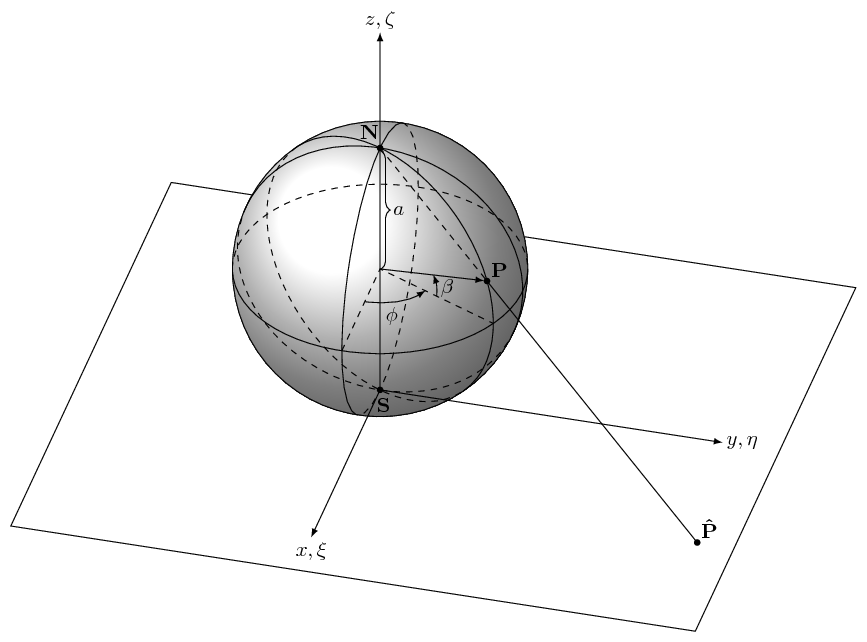
\includegraphics[width=0.8\textwidth]{stereographic_projection.png}
				\caption{\label{fig:stereographic_projection}Stereographic projection}
			\end{figure}
			Given any point $P=(x,y,x)\in S$ other than $N$, we draw the line through $N$ and $P$. We define the stereographic projection of $P$ to be the point $\hat{P} = (\xi,\eta,0)$ where the line intersects the plane at $\zeta = 0$.

			Clearly, $(\xi,\eta,0) = (0,0,1)+ t[(x,y,z)-(0,0,1)]$., where $t$ is given by the fact that $1+t(z-1) = 0$. Solve for $t$:
			\begin{align*}
				t = \frac{1}{1-z}, \mathrm{\:i.e.\:} \hat{P} = \xi + i\eta = \frac{x+iy}{1-z}.\tag*{(2)}
			\end{align*}
			Conversely, given $\hat{P}=\xi+i\eta\in \mathbb{C}\sim(\xi,\eta,0)$, then the line through $N$ and $\hat{P}$ is given by $(x,y,z)=(0,0,1)+t[(\xi,\eta,0)-(0,0,1)],\:t\in \mathbb{R}$. It intersects $S$ when
			\begin{align*}
				\xi^2+\eta^2+\zeta^2=1 &\iff (t\xi)^2+(t\eta)^2+(1-t)^2 = 1\\
				&\iff t^2(\xi^2+\eta^2+\zeta^2) = 2t\\
				&\iff t=0\quad \vee\quad t = \frac{2}{\xi^2+\eta^2+1} = \frac{2}{|\zeta|^2+1}
			\end{align*}
			This corresponds to
			\begin{align*}
				P = \left(\frac{2\xi}{|\zeta|^2+1},\frac{2\eta}{|\zeta|^2+1},\frac{|\zeta|^2+1}{|\zeta|^2+1}\right).
			\end{align*}
			Thus, the stereographic projection $s:S\setminus\{0\}\to \mathbb{C}$ defines a bijection. Letting $\hat{\mathbb{C}}=\mathbb{C}\cup\{\infty\}$ denote the extended complex plane and define $s(N) = \infty$, then $s$ becomes a bijective map $s:S\to\hat{\mathbb{C}}$.\\

			\begin{thm}
				Under stereographic projections, circles on $S$ correspond to circles and lines on $\mathbb{C}$.\\
			\end{thm}

			\begin{rem}
				We refer to circles as lines in $\mathbb{C}$ as 'Circles' in $\hat{\mathbb{C}}$, where lines are considered as circles through '$\infty$'.
			\end{rem}

			\begin{proof}
				The general equation for a circle or line in the plane $\hat{P} = \xi + i \eta$ is as follows:
				\begin{align*}
					A(\xi^2+\eta^2) + B \xi + C \eta + D = 0
				\end{align*}
				Using (2), we get the following:
				\begin{align*}
					&A\left(\left(\frac{x}{1-z}\right)^2+\left(\frac{y}{1-z}\right)^2\right) + 
					B\left(\frac{x}{1-z}\right) + C \left(\frac{y}{1-z}\right) + D = 0 \\ \iff
					&A(x^2+y^2) + Bx(1-z) + Cy(1-z) + D(1-z)^2 = 0 \\ \iff
					&A(1-z)^2 + Bx(1-z) + Cy(1-z) + D(1-z)^2 = 0\\ \iff
					&A(1-z) + Bx + Cy + D(1-z) = 0\\ \iff
					&Bx + Cy + (A-D)z + D+A = 0.
				\end{align*}
				This is the equation for a plane in $\mathbb{R}^3$, which intersects the Riemann-Sphere in a circle.
			\end{proof}
		% subsection stereographic_projections (end)
		\subsection{Möbius Mappings/Transformations} % (fold)
		\label{sub:möbius_mappings_transformations}
			\begin{definition}
				A Möbuis transformation is a mapping on the form
				\begin{align*}
					T(z) = \frac{az+b}{cz+d},\:a,b,c,d\in \mathbb{C}
				\end{align*}
				where $ad-bc\not=0$ (so that $T$ is not constant).

				If $c=0$ we let $T(\infty)= \infty$. Then $T:\hat{\mathbb{C}}\to \hat{\mathbb{C}}$ is bijective. If $c\not=0$, then $T:\mathbb{C}\setminus\{-\frac{d}{c}\}\to \mathbb{C}\setminus\{\frac{a}{c}\}$ is a bijection. Letting $T(- \frac{d}{c}) = \infty$ and $T(\infty) = \frac{a}{c}$ we extend $T$ to a bijective mapping $T:\hat{\mathbb{C}}\to\hat{\mathbb{C}}$.

				\begin{enumerate}
					\item Note that
						\begin{align*}
							T'(z) &= 
							\frac{d}{dz}\left(\frac{az+b}{cz+d}\right) = 
							\frac{a(cz+d)-(az+b)c}{(cz+d)^2}\\ &=
							\frac{ad-bc}{(cz+d)^2}
						\end{align*}
						thus $T:\hat{\mathbb{C}}\to\hat{\mathbb{C}}$ is a conformal mapping.

					\item If
						\begin{align*}
							T(z) &= \frac{ax+b}{cz+d}, \quad S(z) = \frac{\alpha z+\beta}{\gamma z + \delta}\\
							\Rightarrow (S\circ T)(z) &=
							S(T(z)) = 
							\frac{\alpha T(z) + \beta}{\gamma T(z) + \delta} = 
							\frac{\alpha\left(\dfrac{az+b}{cz+d}\right)+\beta}{\gamma\left(\dfrac{az+b}{cz+d}\right) + \delta}\\ &=
							\frac{(\alpha a + \beta c)z + (ab+\beta d)}{(\gamma a + \delta c)z + (\gamma b + \delta d)}
						\end{align*}
						so the composition of Möbius transformations is are Möbius transformations (so they form a group under the operation of composition). Note the following:
						\begin{align*}
							\begin{pmatrix}
								\alpha & \beta\\
								\gamma & \delta
							\end{pmatrix}
							\begin{pmatrix}
								a & b\\
								c & d
							\end{pmatrix} = 
							\begin{pmatrix}
								\alpha a + \beta c & \alpha b + \beta d\\
								\gamma a + \delta c & \gamma b + \delta d
							\end{pmatrix}
						\end{align*}
						Meaning that the composing transformations is 'the same' as multiplying matrices containing the coefficients of the transformations (by 'the same', we mean that there is an isomorphy between these two).

						The inverse, $T^{-1}:\hat{\mathbb{C}}\to \hat{\mathbb{C}}$, is given by solving the following:
						\begin{align*}
							z = T^{-1}(w) =
							\begin{cases}
								- \dfrac{dw+b}{cw+a},  &w\not = \dfrac{a}{c}\\[0.5cm]
								\infty,  &w = \dfrac{a}{c}\\
								- \dfrac{d}{c},  &w = \infty
							\end{cases}
						\end{align*}\\
				\end{enumerate}
			\end{definition}

			\begin{lemma}
				If a Möbius Transformation $T$ has more than 2 fixed points in $\hat{\mathbb{C}}$ (i.e. $z$ s.th. $T(z)=z$) then it is the identity mapping.
			\end{lemma}

			\begin{proof}
				If $c=0$ then
				\begin{align*}
					T(z) &= \frac{az+b}{d}\\
					T(z) &= z \iff \frac{az+b}{c} = z \iff (a-d)z + b = 0
				\end{align*}
				so $T$ has at most one fixed point in $\mathbb{C}$ unless $a=d$ and $b=0$, which is equivalent to $T(z)$ being the identity mapping. This implies that $T$ has at most two fixed points in $\hat{\mathbb{C}}$ unless $T$ is identically 0.

				If $c\not=0$ then
				\begin{align*}
					T(z) = z \iff \frac{az+b}{cz+d}=z \iff az^2+(d-a)z-b = 0.
				\end{align*}
				So $T$ has at most 2 fixed points in $\mathbb{C}$ unless $c=0$ and $a=d$, $b=0$. But $c\not = 0$, which is a contradiction and the result follows.
			\end{proof}

			\begin{thm}
				If $S,T$ are Möbius Transformation s.th. $S(z_i) = T(z_i)$ for three different $z_i$, then $S\equiv T$.
			\end{thm}

			\begin{proof}
				$T^{-1}\circ S^{-1}$ is a Möbius Transformation s.th. $(T^{-1}\circ S)(z_i) = z_i,\:i=1,2,3$. This implies that $(T^{-1}\circ S)(z) = z,\:\forall z$ by lemma. So $S\equiv T$.
			\end{proof}
		% subsection möbius_mappings_transformations (end)
	% section conformal_mappings_and_stereographic_projections (end)
	\section{More on Möbius Transformations} % (fold)
	\label{sec:more_on_möbius_transformations}
		Recall that a Möbius transformation is a mapping on the form
		\begin{align*}
			T(z) = \frac{az+b}{cz+d},\:a,b,c,d \in \mathbb{C},\: ad-bc\not=0.
		\end{align*}
		Some particular cases:
		\begin{enumerate}
			\item $T(z) = z+b$; a translation
			\item $T(z) = az = |a|e^{i\arg(z)}$; a rotation \& magnification
			\item $T(z) = \frac{1}{z}$; an inversion  
		\end{enumerate}
		Note that if $c\not=0$,
		\begin{align*}
			T(z) = \frac{az+b}{cz+d} = \frac{\frac{a}{c}(cz+d)-\frac{ad}{c}+b}{cz+d} = \frac{a}{c} - \frac{ad-bc}{c^2}\frac{1}{z+\frac{d}{c}}
		\end{align*}
		so every Möbius transformation is a composition of Möbius transformation of the type 1, 2, or 3.

		\begin{thm}
			Every Möbius transformation maps 'circles' onto 'circles'\\
		\end{thm}

		\begin{rem}
			Recall that a 'circle' in $\hat{\mathbb{C}}$ is a circle or a line in $\mathbb{C}$. A line in $\mathbb{C}$ is a 'circle' through $\infty$ in $\hat{\mathbb{C}}$.\\
		\end{rem}

		\begin{proof}
			It is easy to see that mappings on the form of 1 or 2 map circles onto circles and lines onto lines. It is enough to prove that inversion
			\begin{align*}
				T(z) = \frac{1}{z} = \frac{1}{x+iy} = \frac{x+iy}{x^2+y^2} = \frac{x}{x^2+y^2}+ i \frac{-y}{x^2+y^2} = u+iv
			\end{align*}
			maps 'circles' onto 'circles'. [Note that $u^2+v^2 = \frac{1}{x^2+y^2}$].

			A 'circle' in $\hat{\mathbb{C}}$ has equation
			\begin{align*}
				 A(x^2+y^2) + Cx + Dy + E = 0 &\iff 
				 A + \frac{Cx}{x^2+y^2} + \frac{Dy}{x^2+y^2} + \frac{E}{x^2+y^2} = 0\\ &\iff
				 A + Cu + Dv + E(u^2+v^2);
			\end{align*}
			Which is precisely the equation of a 'circle' in $\hat{\mathbb{C}}$.
		\end{proof}

		\begin{example}
			Determine the image of the disk $|z-2|=2$ under the transformation $T(z) = \dfrac{z}{2z-8}$.

			Solution: First determine the image of $c: |z-2|=2$.
			\begin{align*}
				T(4) &= \infty\Rightarrow \text{$T(z)$ must be a line}\\
				T(0) &= 0,\quad T(2+2i) = \frac{2+2i}{2(2+2i)-8} = \frac{2+2i}{-4+2i} = -\frac{1}{2}\frac{1+i}{1-i} = - \frac{i}{2}.
			\end{align*}
			Since $T(2) = -\frac{1}{2}$, clearly $\{z:|z-2|<2\}$ maps to the left half-plane.
		\end{example}

		Given a 'circle' $C_z$ in the $z$-plane, and a 'circle' $C_w$ in the $w$-plane, can one find a Möbius transformation $T$ s.th. $T(C_z) = C_w$? Yes!
		\subsection{The Cross-Ratio} % (fold)
		\label{sub:the_cross_ratio}
			\begin{definition}
				Let $z_1,z_2,z_3\in\hat{\mathbb{C}}$ be distinct points. Put 
				\begin{align*}
					(z,z_1,z_2,z_3):= \frac{z-z_1}{z-z_3}\frac{z_2-z_3}{z_2-z_1}\in\hat{\mathbb{C}}.
				\end{align*}
				If some of the $z_i$ is infinity, then the right-hand side should be interpreted as
				\begin{align*}
					(z,z_1,z_2,z_3) = 
					\begin{cases}
						\dfrac{z_2-z_3}{z-z_3} &z_1=\infty\\[0.3cm]
						\dfrac{z-z_1}{z-z_3} &z_2=\infty\\[0.3cm]
						\dfrac{z-z_1}{z_2-z_1} &z_3=\infty
					\end{cases}
				\end{align*}
			\end{definition}
			$(z,z_1,z_2,z_3)$ is called the cross-ratio of the points. Note that $S(z):=(z,z_1,z_2,z_3)$ is a Möbius transformation s.th. $S(z_1) =0,\:S(z_2) = 1,\:S(z_3)=\infty$.

			By an earlier proposition, it is the unique Möbius transformation that maps $z_1,z_2,z_3$ to 0,1,$\infty$.\\

			\begin{thm}
				Given a triple $z_1,z_2,z_3\in\hat{\mathbb{C}}$ of distinct points, and another triple $w_1,w_2,w_3\in\hat{\mathbb{C}}$ of distinct points, there is a unique Möbius transformation $T$ s.th. $T(z_i) = w_i,\:i=1,2,3$.
			\end{thm}

			\begin{proof}
				By our earlier proposition, there is at most one such $T$. We now prove that there is a unique such $T$ by constructing a Möbius transformation $T$ s.th. $T(z_i) = w_i$. Put $S(z) = (z,z_1,z_2,z_3)$, $U(w) = (w,w_1,w_2,w_3)$.
				\begin{align*}
					S(z_1) &\longrightarrow 0 \longleftarrow U(w_1)\\
					S(z_2) &\longrightarrow 1 \longleftarrow U(w_2)\\
					S(z_3) &\longrightarrow \infty \longleftarrow U(w_3)
				\end{align*}
				So the transformation $T(z):=(U^{-1}\circ S)(z) = U^{-1}(S(z))$. Furthermore
				\begin{align*}
					w=T(z) &\iff U^{-1}(S(z)) = w \iff U(w) = S(z) \\ &\iff
					(z,z_1,z_2,z_3) = (w,w_1,w_2,w_3).
				\end{align*}
			\end{proof}

			Let $z_1,z_2,z_3$ be three distinct points on a 'circle' $C_z$ in $\hat{\mathbb{C}}$. Note that $C_z$ is \textit{oriented} by the order of $z_1,z_2,z_3$. that is, $C_z$ is acquiring an orientation by proceeding through $z_1,z_2,z_3$ in succession.

			Since Möbius transformations are conformal, it maps the ragion to the left of $C_z$ oriented by $z_1,z_2,z_3$ onto the region to the left of $C_w=T(C_z)$, if oriented by $w_1,w_2,w_3$.\\

			\begin{example}
				Find a Möbius transformation that maps the region $|z|>1$ onto $\Re(w)<0$

				Solution: Let $z_1=1$, $z_2 = -i$, $z_3 = -1$, and $w_1 = 0$, $w_2 = 1$, $w_3 = \infty$.
				\begin{align*}
					\frac{w-w_1}{w-\infty}\frac{i-\infty}{i-0} &= \frac{z-1}{z+1}\frac{-i+1}{-i-1} \\\iff
					w &= (-i)\frac{z-1}{z+1}\frac{1-i}{1+i} = \frac{1-z}{1+z}.
				\end{align*}
			\end{example}
		% subsection the_cross_ratio (end)
		\subsection{Symmetry preserving property} % (fold)
		\label{sub:symmetry_preserving_property}
			Two points $z_1,z_2$ are said to be symmetric w.r.t. a line $L$ if $L$ is the perpendicular bisector of the line segment from $z_1$ to $z_2$. This means that every circle or line through the points $z_1$ and $z_2$ intersect $L$ orthogonally. This motivates the following definition:\\

			\begin{definition}
				Two points are said to be symmetric w.r.t. a circle if every circle or line through $z_1,z_2$ intersects the circle orthogonally. In particular, the center of the circle and $\infty$ are symmetric w.r.t the circle.\\
			\end{definition}

			\begin{thm}[Symmetry Principle]
				Let $C_z$ be a circle or line in the $z$-plane and $w=T(z)$ be a Möbius transformation. Then the two points $z_1,z_2$ are symmetric w.r.t $C_z$ iff.
				\begin{align*}
					w_1 = T(z_1)\text{ and } w_2=T(z_2)\text{ are symmetric w.r.t. $C_w=T(C_z)$}.
				\end{align*}
			\end{thm}

			\begin{proof}
				Follows since Möbius transformations preserve the class of circles and lines as well as orthogonality.\\
			\end{proof}

			\begin{example}
				Let $C$ be a proper circle in $\mathbb{C}$ with center $a$ and radius $R$. Given a point $\alpha\in\hat{\mathbb{C}}$ there is a unique point $\alpha^*$ s.th. $\alpha$ and $\alpha^*$ are symmetric w.r.t $C$. Indeed it holds that
				\begin{align*}
					(\alpha^*-\alpha)\overline{(\alpha- \alpha^*)} = R^2
				\end{align*}
				or
				\begin{align*}
					\alpha^* = \alpha + \frac{R^2}{\overline{(\alpha- a)}} = a + \frac{R^2}{|\alpha-a|^2}(\alpha-a)
				\end{align*}
			\end{example}
			Note: $\arg(\alpha^*- \alpha) = \arg(\alpha-a)$. $|\alpha^*- a||\alpha-a| = R^2$.
		% subsection symmetry_preserving_property (end)
	% section more_on_möbius_transformations (end)
	\section{Dirichlet's Problem} % (fold)
	\label{sec:dirichlet_s_problem}
		Many applications involve solving Dirichlet's problem: Find a function $\varphi(x,y)$ defined on $D\cup\partial D$, $\varphi\in C^2$ in $D$ s.th.
		\begin{enumerate}
			\item $\Delta \varphi = \varphi_{xx}+\varphi_{yy} = 0$ in $D$
			\item $\varphi =$ some given function on $\partial D$.
		\end{enumerate}
		This problem is easily solved in some special cases.
		% \begin{multicols*}{2}
			\begin{enumerate}
				\item 
					If the region we are interested in is the area between two points on the $x-$axis, and the temperature at the endpoints are given as $A$ and $B$, then 
					\begin{align*}
						\begin{cases}
							\Delta \varphi = 0 \text{ in } D\\
							\varphi(a,y) = A\\
							\varphi(x,b) = B
						\end{cases}
					\end{align*}
					Let $\varphi(x,y) = \alpha x+\beta$, choose 
					\begin{align*}
						\begin{cases}
							\alpha a + \beta = A\\
							\alpha b + \beta = B
						\end{cases}\iff
						\begin{cases}
							\alpha = \dfrac{B-A}{b-a}\\[0.3cm]
							\beta = \dfrac{Ab-Ba}{b-a}
						\end{cases}
					\end{align*}
					So $\varphi(x,y) = \dfrac{A-B}{b-a}x + \dfrac{Ab-Ba}{b-a}$.

				\item 
					If the region we are interested in is say, the right half-plane, and the temperature at some point on the positive imaginary axis is given as $A$, and the temperature at some point on the negative imaginary axis is given as $B$, then
					\begin{align*}
						&\varphi(x,y) = \alpha \mathrm{Arg}(z)+\beta. \text{ choose $\alpha$, $\beta$ s.th.}\\&
						\begin{cases}
							\alpha\cdot\frac{\pi}{2}+\beta = A\\
							\alpha\cdot - \frac{\pi}{2} + \beta = B
						\end{cases}\iff
						\begin{cases}
							\alpha = \dfrac{A-B}{\pi}\\[0.3cm]
							\beta = \dfrac{A+B}{2}.
						\end{cases}\\\\
						&\varphi(x,y) = \frac{A-B}{\pi}\mathrm{Arg}(z) + \frac{A+B}{2}.
					\end{align*}

				\item 
					If the region we are interested in lies between the positive real axis and a ray centered at the origin with argument $\alpha$ relative to the positive real axis
					\begin{align*}
						\varphi(x,y) = \frac{1}{\alpha}\mathrm{Arg}(z).
					\end{align*}

				\item 
					If the region is the upper half-plane, and given a set of $n$ ordered points $x_i$ on the real axis, the temperature between the points $x_i,\:x_{i+1}$ is given by $a_i$. Then the temperature distribution is given by
					\begin{align*}
						\varphi(x,y) = a_n + \frac{1}{\pi}\sum\limits_{i=1}^{n}(a_{i-1}-a_i)\mathrm{Arg}(z-x_i)
					\end{align*}

				\item 
					If the region is an annulus with inner radius $r_1$ and outer radius $r_2$, and the temperature at these are $A$ and $B$ respectively, then the temperature distribution is given by
					\begin{align*}
						\varphi(x,y) = \alpha\ln|z] + \beta,\quad \alpha=\frac{B-A}{\ln(r_r)-\ln(r_1)},\quad \beta = \frac{A\ln(r_2)-B\ln(r_1)}{\ln(r_2)-\ln(r_1)}.
					\end{align*}
			\end{enumerate}

			How about more complicated Dirichlet problems? The idea is to map the more complicated problem to an easier problem using a conformal mapping, e.g. Möbius transformations.\\

			\begin{thm}
				Suppose $f:D\to D'$ is analytic, $f=u+iv$, where $D,\:D'$ are domains. If $\psi(u,v)$ is harmonic in $D'$, then $\phi(x,y):=\phi(u(x,y),v(x,y))$ (*) is harmonic.
			\end{thm}

			\begin{proof}
				Take $z_0\in D$, then $w_0=f(z_0)\in D'$, and since $D'$ is open, there exists a disk $V\ni w_0$ s.th. $v\subseteq D'$. Since $f$ is continuous we know that there is a disk $U\in D$ s.th. $f(U)\subseteq V$. Since $\psi$ is harmonic in $D'$ which is simply connected, there is an analytic functions in $V$ s.th. $\psi = \Re(g)$. But then $g\circ f$ is analytic in $U$ and moreover $\Re(g\circ f)(z) = \psi(u(x,y),v(x,y)) = \phi(x,y)$. Hence $\phi$ is harmonic in $U$. Since $z_0$ was chosen arbitrarily, this implies that $phi$ is harmonic in $D$.
			\end{proof}

			Suppose now that the function $f_D\to D'$ maps $D$ bijectively on $D'$ and that $\partial D$ maps bijectively onto $\partial D'$. . Suppose also that the boundary conditions for $\psi$ in $D'$ correspond to the boundary conditions for $\phi$ in $D$, i.e. (*) holds for $(x,y)\in\partial D$.

			If we can solve the Dirichlet problem for $\psi\in D'$, we can also solve it for $\phi$. \\

			\begin{example}
				Find a function $\phi$ which is harmonic inside the unit disk $|z|<1$ s.th. $\phi(x,y)=1$ on the upper half-circle and $-1$ on the lower half-circle.

				Solution: The Möbius transformation taking
				\begin{align*}
					\begin{cases}
						-1	&\to 0\\
						0	&\to 1\\
						1	&\to \infty
					\end{cases}
					\quad\text{is given by}\quad 
					\frac{w-0}{w-\infty}\frac{1-\infty}{1-0} &= \frac{z+1}{z-1}\frac{0-1}{0+1}\\
					w = - \frac{z+1}{z-1} &= \frac{1+z}{1-z}.
				\end{align*}
				\begin{align*}
					\Rightarrow \psi(u,v) &= \frac{2}{\pi}\mathrm{Arg}(w)\\
					\Rightarrow \phi(x,y) &= \frac{2}{\pi}\mathrm{Arg}\left(\frac{1+z}{1-z}\right) = 
					\frac{2}{\pi}\mathrm{Arg}\left(\frac{1+x+iy}{1-x-iy}\right) = 
					\mathrm{Arg}\left(\frac{2y}{1-x^2-y^2}\right)\\
				\end{align*}
			\end{example}

			\begin{thm}[The Riemann Mapping Theorem]
				Every simply connected domain $D\not= \mathbb{C}$ can be conformally mapped onto the open unit disk.\\
			\end{thm}

			\begin{thm}[Poisson Integral Formula for the disk]
				Let $f$ be a continuous function defined on the unit circle $|z|=1$. Then
				\begin{align*}
					u(re^{i\theta}) = \int\limits_{0}^{2\pi}\frac{1-r^2}{1-2r\cos(\theta-t)+r^2}f(e^{it})dt
				\end{align*}
			\end{thm}

			\begin{proof}
				will follow from the Cauchy Integral Formula.
			\end{proof}
	% section dirichlet_s_problem (end)
	\section{Complex Integration} % (fold)
	\label{sec:complex_integration}
		We shall now study so-called contour integral (or line integrals) of complex-valued functions. This theory of integration will teach more about the properties of analytic functions. There are infinitely many parameterizations for a given curve, e.g. change the 'direction'. Obviously, there are two natural directions of a smooth curve. A smooth curve with a specified directions is called a directed smooth curve.\\

		\begin{example}
			Give parameterizations of the following directed smooth curves
			\begin{enumerate}[label=(\alph*)]
				\item The line from $z_1$ to $z_2$.
				\item The circle if radius $r$ and $z_0$
			\end{enumerate}

			\begin{enumerate}[label=(\alph*)]
				\item $z(t) = z_1 + t(z_2-z_1),\:0\le t \le 1$
				\item $z(t) = z_0 + re^{it},\: 0\le t\le 2\pi$\\
			\end{enumerate}
		\end{example}

		\begin{definition}
			A contour $\gamma$ is either a single point or a finite sequence $(\gamma_1,\gamma_2,\ldots,\gamma_n)$ of oriented smooth curves s.th. the terminal point of the $k^{\mathrm{th}}$ curve is the starting point of the $k+1^{\mathrm{th}}$ curve. The contour $\gamma$ is said to be a closed contour if the terminal and initial points coincide. If these are the only self-intersections, we call $\gamma$ a simple closed curve.
		\end{definition}

		If $\gamma$ is a smooth curve, the length of $\gamma$ is given by
		\begin{align*}
			l(\gamma) = 
			\int\limits_{a}^{b}\sqrt{\left(\frac{dx}{dt}\right)^2+\left(\frac{dy}{dt}\right)^2}dt = 
			\int\limits_{a}^{b}\left|\frac{dz}{dt}\right| dt
		\end{align*}

		\subsection{Contour Integrals} % (fold)
		\label{sub:contour_integrals}
			We shall now see how to define the contour integral of a complex-valued function over a contour $\gamma$
			\begin{align*}
				\int\limits_{\gamma}f(z)dz
			\end{align*}
			where $\gamma$ is a  smooth curve.\\

			\begin{definition}[Properties of Contour Integrals]
			~\\
				\begin{itemize}
					\item $\displaystyle\int\limits_{\gamma}(f+g)(z)dz = \int\limits_{\gamma}f(z)dz + \int\limits_{\gamma}g(z)dz$
					\item $\displaystyle\int\limits_{\gamma}cf(z) = = c\int\limits_{\gamma}f(z)dz$
					\item $\displaystyle\int\limits_{-\gamma}f(z)dz = -\int\limits_{\gamma}f(z)dz$\\
				\end{itemize}
			\end{definition}

			\begin{thm}
			\label{thm:integrability}
				If $f$ in continuous along $\gamma$, then $f$ is integrable.
			\end{thm}

			How do we compute it? First consider a segment of $\mathbb{R}$
			\begin{align*}
				\int\limits_{a}^{b}f(t)dt,\quad f=u+iv
			\end{align*}
			and $u,\:v$ continuous on $[a,b]$. Let $F(t)$ be an anti-derivative of $f(t)$, i.e. $F(t) = U(t)+iV(t)$, where $U'(t) = u(t)$ and $V'(t) = v(t)$, so
			\begin{align*}
				\int\limits_{a}^{b}f(t)dt = 
				\int\limits_{a}^{b}u(t)+iv(t)dt =
				\int\limits_{a}^{b}u(t)dt +
				i\int\limits_{a}^{b}v(t)dt =
				\left[U(t)\right]_a^b + i\left[V(t)\right]_a^b = F(b)-F(a).\\
			\end{align*}

			\begin{thm}
				If $f$ is continuous on $[a,b]$ and $F'(t)=f(t)$ for $t\in[a,b]$, then
				\begin{align*}
					\int\limits_{a}^{b}f(t)dt = F(b)-F(a)
				\end{align*}
			\end{thm}

			The integral along any directed smooth curve can be reduced to an integral on the above form by using a parameterization of the directed smooth curve $z(t,\: a\le t \le b)$.

			Let $z_0 = z(t_0),\:z_1=z(t_1),\ldots,z_n = z(t_n)$, where $a=t_0<t_1<t_2<\ldots<t_n=b$. then
			\begin{align*}
				\sum\limits_{k=1}^{n}f(z_k)\Delta z_k &=
				\sum\limits_{k=1}^{n}f(z(t_k))(z(t_k)-z(t_{k-1}))\tag*{Riemann sum for $f(z(t))z'(t)$}\\ &=
				\sum\limits_{k=1}^{n}f(z(t_k))z'(t_k)\Delta t_k
			\end{align*}
			This suggests the following theorem:\\

			\begin{thm}
				Let $f$ be a continuous function on a directed smooth curve having admissible parameterization $z(t),\:a\le t\le b$. Then
				\begin{align*}
					\int\limits_{\gamma}f(z)dx = \int\limits_{a}^{b}f(z(t))z'(t)dt.\\
				\end{align*}
			\end{thm}

			\begin{example}
				compute
				\begin{align*}
					\int\limits_{C_r}(z-z_0)^ndz, \:n\in \mathbb{Z}
				\end{align*}
				over $C_r=\{z:|z-z_0|=r\}$, oriented counter-clockwise.

				Solution: Let $z(t)=re^{it},\:0\le t\le 2\pi$. then $z'(t)=ire^{it}$, so
				\begin{align*}
					\int\limits_{C_r}(z-z_0)^ndz &= 
					\int\limits_{0}^{2\pi}r^ne^{it}ire^{it}dt =
					ir^{n+1}\int\limits_{0}^{2\pi}e^{i(n+1)t}dt\\ &=
					\begin{cases}
						ir^{n+1}\left[\dfrac{e^{i(n+1)t}}{i(n+1)}\right]_0^{2\pi}, &n\not=-1\\[0.3cm]
						i2\pi, &n=-1
					\end{cases}\\
				\end{align*}

				\begin{definition}
					Suppose $\gamma=\gamma_1+\gamma_2+\ldots+\gamma_n$ and let $f$ be continuous on $\gamma$, then we let
					\begin{align*}
						\int\limits_{\gamma}f(z)dz = \sum\limits_{k=1}^{n}\int\limits_{\gamma_k}f(z)dz\tag*{and if $\gamma=z_0$ the integral vanishes identically.}\\
					\end{align*}
				\end{definition}
			\end{example}
		% subsection contour_integrals (end)

		\subsection{ML-Inequality} % (fold)
		\label{sub:ml_inequality}
			Suppose $|f(z)\le M\:\forall Z\in \gamma$. Then
			\begin{align*}
				\left|\sum\limits_{k=1}^{n}f(z_k)\Delta z_k\right| \le
				\sum\limits_{k=1}^{n}\left|f(z_k)\Delta z_k\right| \le
				M\sum\limits_{k=1}^{n}\left|\Delta z_k\right| \le
				M l(\gamma).
			\end{align*}
			Letting $\mu(P_n)\to 0$ leaves us with
			\begin{align*}
			\left|\int\limits_{\gamma}f(z)dz\right|\le ML,\: L=l(\gamma)
			\end{align*}


		\begin{thm}
			Suppose $f$ is continuous on $\gamma$ and that $|f(z)|\le M\:\forall z\in \gamma$. Then
			\begin{align*}
				\left|\int\limits_{\gamma}f(z)dz\right|\le ML,\: L=l(\gamma)
			\end{align*}
		\end{thm}
		% subsection ml_inequality (end)
	% section complex_integration (end)
	\section{Independence of Path, Cauchy's Integral Theorem} % (fold)
	\label{sec:independence_of_path_cauchy_s_integral_theorem}
		\subsection{Independence of Path} % (fold)
		\label{sub:independence_of_path}
			\begin{thm}
				Suppose the $f$ is continuous in a domain $D$, and that $f$ has an anti-derivative $F$ in $D$, i.e. $F'(z) = f(z)\:\forall z\in D$. Let $\gamma$ be a contour in $D$ with initial point $z_i$ and terminal points $z_t$. Then
				\begin{align*}
					\int\limits_{\gamma}f(z)dz = F(z_t)-F(z_i)
				\end{align*}
			\end{thm}

			\begin{proof}
				\begin{align*}
					\int\limits_{\gamma}f(z)dz =
					\sum\limits_{k}\int\limits_{\gamma_k}f(z)dz =
					\sum\limits_k \int\limits_{\tau_{k-1}}^{\tau_k}f(z(t))z'(t) dt
				\end{align*}
				where $z(t),\: \tau_{k-1}\le t\le \tau_k$ is a parameterization of $\gamma_k$. Now, $\frac{d}{dt}F(z(t)) = F'(z(t))z'(t)=f(z(t))z'(t)$. So by Theorem~\ref{thm:integrability} from the previous chapter, 
				\begin{align*}
					\int\limits_{\tau_{k-1}}^{\tau_k}f(z(t))z'(t)dt =
					\left[F(z(t))\right]_{\tau_{k-1}}^{\tau_k} = F(z(\tau_k)) - F(z(\tau_{k-1})).
				\end{align*}
				Summing over $k$ yields our result.\\
			\end{proof}

			\begin{example}
				\begin{multicols}{2}
					Compute
					\begin{align*}
						\int\limits_{\gamma}\cos(z)dz
					\end{align*}
					with $\gamma$ as in figure.
					\begin{figure}[H]
						\begin{tikzpicture}[scale = 0.7, transform shape]
							\begin{axis}
								[
								% height = \textwidth,
								% width = \textwidth,
								ymin = -1, ymax = 2,
								xmin = -2, xmax = 2,
								ytick = {-1,1},
								xtick= {-2,-1,1,2},
								% xlabel = $\mathfrak{Re}$,
								% ylabel = $\mathfrak{Im}$,
								tikzDefaults,
								]

								\addplot[thick, domain=0:pi]({cos(deg(x))},{sin(deg(x))});
								\addplot[thick, domain=1:2]{x-1};
							\end{axis}
						\end{tikzpicture}
					\end{figure}
				\end{multicols}
				Solution:
				\begin{align*}
					\int\limits_{\gamma}\cos(z)dz = \left[\sin(z)\right]_{-1}^{2+i} = \sin(2+i)-\sin(-1).\\
				\end{align*}
			\end{example}

			\begin{cor}
				If $f$ is continuous in a domain $D$ and has an anti-derivative in $D$, then
				\begin{align*}
					\int\limits_{\gamma}f(z)dz = 0
				\end{align*}
				for any closed contour $\gamma\in D$.\\
			\end{cor}

			\begin{example}
				Let $f(z)=z^n,\:n\not=1$, and let $\gamma$ be any closed contour not passing through the origin. Then
				\begin{align*}
					\int\limits_{\gamma}z^n dz = 0
				\end{align*}
				since $z^n$ has an anti-derivative $\frac{z^{n+1}}{n+1}$ in $\mathbb{C}\setminus\{0\}$.\\
			\end{example}

			\begin{thm}
				Let $f$ be continuous in a domain $D$. Then the following are equivalent:
				\begin{enumerate}[label=(\roman*)]
					\item $f$ has an anti-derivative in $D$.
					\item $\displaystyle\int\limits_{\gamma}f(z)dz=0$ for every closed contour $\gamma\in D$.
					\item Contour integrals are independent of path in $D$. (i.e. if $\gamma_1$ and $\gamma_2$ are two contours with the same initial and terminal points, then the integrals give the same value).
				\end{enumerate}
			\end{thm}

			\begin{proof}
			~\\
				\begin{itemize}
					\item [$(i)\Rightarrow(ii)$] Shown above.
					\item [$(i)\Rightarrow(iii)$] Shown above.
					\item [$(ii)\Rightarrow(iii)$] Given $\gamma_1$ and $\gamma_2$, let $\gamma:=\gamma_1+(-\gamma_2)\Rightarrow$ the integral is identically zero.
					\item [$(iii)\Rightarrow(i)$] Fix $z_0\in D$. This implies that for any $z\in D$ there exists a polygonal path $\gamma_z$ from $z_0$ to $z$. Define $F(z) = \displaystyle\int\limits_{\gamma_z}f(\zeta)d \zeta$. $F(z)$ is well-defined, i.e. independent of choice of $\gamma_z$, by $(iii)$.
					\begin{align*}
						\Rightarrow F(z+\Delta z) - F(z) &= 
						\int\limits_{L}f(\zeta)d \zeta = 
						\int\limits_{L}f(z)d \zeta + \int\limits_{L}(f(\zeta)-f(z))d \zeta\\ &=
						f(z)\Delta z + \int\limits_{L}(f(\zeta)-f(z))d \zeta
						\intertext{i.e.}
						\frac{F(z+\Delta z)-F(z)}{\Delta z} &= 
						f(z) + \frac{1}{\Delta z}\int\limits_{L}(f(\zeta)-f(z))d \zeta
					\end{align*}
					But by the ML-Inequality
					\begin{align*}
						\left|\frac{1}{\Delta z}\int\limits_{L}(f(\zeta)-f(z))d \zeta\right| \le
						\frac{1}{\Delta z}\max\limits_{\zeta\in L}|f(\zeta)-f(z)| |\Delta z|\to 0
					\end{align*}
					as $\Delta z\to 0$ by the continuity of $f$. This implies that $F'(z)=f(z)$.
				\end{itemize}
			\end{proof}
		% subsection independence_of_path (end)
		\subsection{Cauchy's Integral Theorem} % (fold)
		\label{sub:cauchy_s_integral_theorem}
			Let $\gamma$ be a simple closed contour in $\mathbb{C}$ parameterized by $z(t),\:a\le t\le b$.
			\begin{align*}
				\Rightarrow \int\limits_{\gamma}f(z)dz &= 
				\int\limits_{a}^{b}f(z(t))z'(t)dt = 
				\int\limits_{a}^{b}[u(x(t),y(t))+iv(x(t),y(t))]\left(\frac{dx}{dt}+i \frac{dy}{dt}\right)dt \\ &=
				\int\limits_{a}^{b}\left[u(x(t),y(t))\left(\frac{dx}{dt}\right)-v(x(t),y(t))\left(\frac{dy}{dt}\right)\right]dt\\ &+
				i\int\limits_{a}^{b}\left[v(x(t),y(t))\left(\frac{dx}{dt}\right)-u(x(t),y(t))\left(\frac{dy}{dt}\right)\right]dt
				\intertext{i.e.}
				\int\limits_{\gamma}f(z)dz &=
				\int\limits_{\gamma}udx-vdy + i\int\limits_{\gamma}vdx+udy.
			\end{align*}

			\begin{thm}[Green's Theorem]
				Let $\vec{F}(x,y)=(F_1(x,y),F_2(x,y))$ be a $C^1$ vector field defined on a simply connected domain $D$, and let $\gamma$ be a positively oriented simple closed contour in $D$. Then
				\begin{align*}
					\int\limits_{\gamma}(F_1dx+F_2dy) = 
					\iint\limits_{\Omega}\left(\frac{\partial F_2}{\partial dx}- \frac{\partial F_1}{\partial dy}\right)dxdy
				\end{align*}
				Where $\gamma = \partial \Omega$. 
			\end{thm}

			Let us use this expression for the integral of $f(z)$ over $\gamma$:
			\begin{align*}
				\int\limits_{\gamma}f(z)dz = 
				\iint\limits_{\Omega}\left(- \frac{\partial v}{\partial x}- \frac{\partial u}{\partial y}\right)dxdy +
				i \iint\limits_{\Omega}\left(\frac{\partial u}{\partial x}- \frac{\partial y}{\partial y}\right)dxdy.
			\end{align*}
			If we assume $u,v\in C^1$. If we moreover assume that $f$ is analytic in $D$, the entire integral vanishes identically in view of the Cauchy-Riemann Equations.\\

			\begin{thm}[Cauchy's Integral Theorem]
				Suppose that $f$ is analytic in a simply connected domain $D$ and let $\gamma$ be any closed contour in $D$. Then
				\begin{align*}
					\int\limits_{\gamma}f(z)dz = 0\\
				\end{align*}
			\end{thm}

			\begin{rem}
				The theorem generalizes the discussion thus far in two ways:
				\begin{enumerate}[label=(\roman*)]
					\item $\gamma$ can be any closed contour, i.e. need not be simple.
					\item The assumption that $u,v\in C^1$ has been dropped.
				\end{enumerate}

				The fact that the second assumption can be dropped was proven by Edward Goursat. The Theorem is therefore often called the Cauchy-Goursat Theorem.\\
			\end{rem}

			\begin{rem}
				The Theorem implies that if $f$ is analytic inside and on a simple closed contour, then the integral of $f$ along said contour is identically zero.\\
			\end{rem}

			\begin{thm}
				Suppose $f$ is analytic in a simply connected domain. Then $f$ has an anti-derivative, contour integrals are path-independent, and integrals over closed contours vanish identically.\\
			\end{thm}

			\begin{example}
				\begin{multicols}{2}
					Consider the contours $\gamma$ (black) and $\gamma'$ (dashed) in the figure. Suppose that $f$ is analytic in a domain containing $\gamma$ and $\gamma'$, and the region between these two contours. (In the equations below, $\gamma_1,\:\gamma'_1$ denote the parts of the contours 'above' $\rho_1,\:\rho_2$ and $\gamma_2,\:\gamma'_2$ denote the parts of the contours 'below' $\rho_1,\:\rho_2$). By Cauchy's Integral Theorem
					\begin{figure}[H]
					\flushright
						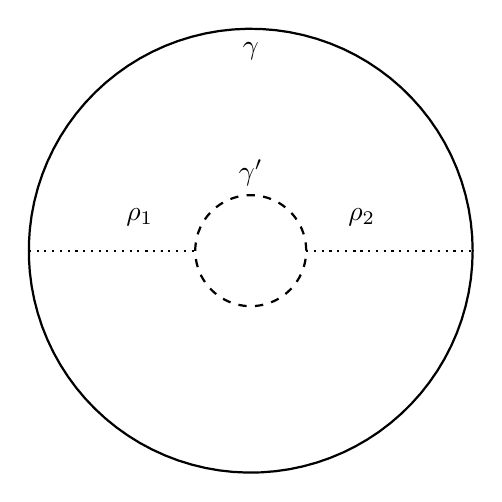
\begin{tikzpicture}
							\begin{axis}
								[
								% height = \textwidth,
								% width = \textwidth,
								ymin = -2.02, ymax = 2.02,
								xmin = -2.02, xmax = 2.02,
								ytick = \empty,
								xtick= \empty,
								% xlabel = $\mathfrak{Re}$,
								% ylabel = $\mathfrak{Im}$,
								tikzDefaults,
								axis equal image,
								axis lines = none,
								]

								\addplot[thick, dashed, samples=100, domain=0:2*pi]
									({0.5*cos(deg(x))},{0.5*sin(deg(x))}) node at (axis cs:0,0.7) {$\gamma'$};

								\addplot[thick, samples=100, domain=0:2*pi]
									({2*cos(deg(x))},{2*sin(deg(x))}) node at (axis cs:0,1.8) {$\gamma$};

								\addplot[thick, dotted, domain=-2:-0.5]
									{0} node at (axis cs:-1,0.3) {$\rho_1$};
								\addplot[thick, dotted, domain=0.5:2]
									{0} node at (axis cs:1,0.3) {$\rho_2$};
							\end{axis}
						\end{tikzpicture}
					\end{figure}
				\end{multicols}
				\begin{align*}
						\int\limits_{\gamma_1} &+ 
						\int\limits_{\rho_1} + 
						\int\limits_{-\gamma'_1}+
						\int\limits_{\rho_2} = 0\quad\quad\quad
						\int\limits_{\gamma_2} + 
						\int\limits_{\rho_2} + 
						\int\limits_{-\gamma'_2}+
						\int\limits_{\rho_1} = 0
					\end{align*}
					\begin{align*}
						\Rightarrow \int\limits_{\gamma_1} + \int\limits_{\gamma_2} &=
						 \int\limits_{-\gamma'_1} + \int\limits_{-\gamma'_2} \\
						 \int\limits_{\gamma} &= \int\limits_{\gamma'}.
					\end{align*}
			\end{example}
			So we can 'deform' the contour $\gamma$ into $\gamma'$ without affecting the integral. This illustrates the 'Deformation Theorem'.
		% subsection cauchy_s_integral_theorem (end)
	% section independence_of_path_cauchy_s_integral_theorem (end)
	\section{Cauchy's Integral Formula and Applications} % (fold)
	\label{sec:cauchy_s_integral_formula_and_applications}
		\begin{thm}[Cauchy's Integral Formula]
			Suppose $f$ is analytic in a simply connected domain $D$. Let $\gamma$ be a simple closed positively oriented contour in $D$. Moreover, let $z_0\in \gamma$. then
			\begin{align*}
				f(z_0) = \frac{1}{2\pi i}\int\limits_{\gamma}\frac{f(z)}{z-z_0}dz.
			\end{align*}
		\end{thm}

		\begin{proof}
			$\displaystyle \frac{f(z)}{z-z_0}$ is analytic in $D\setminus\{z_0\}$. As in the last example from the previous chapter, we see that
			\begin{align*}
				\int\limits_{\gamma}\frac{f(z)}{z-z_0}dz &= 
				\int\limits_{C_r}\frac{f(z)}{z-z_0}dz =
				\int\limits_{C_r}\frac{f(z_0)}{z-z_0}dz +
				\int\limits_{C_r}\frac{f(z)-f(z_0)}{z-z_0}dz \\ &=
				2\pi i f(z_0) + \int\limits_{C_r}\frac{f(z)-f(z_0)}{z-z_0}dz.
			\end{align*}
			Note: Clearly, the second term above is independent of $r$. So it is enough to show that
			\begin{align*}
				\lim\limits_{r\to 0}\int\limits_{C_r}\frac{f(z)-f(z_0)}{z-z_0}dz = 0.
			\end{align*}
			Let $M_r:=\max\limits_{z\in C_r}|f(z)-f(z_0)|$. $f$ is continuous, which implies that $M_r\to 0$ as $r\to 0^+$. So, by the ML-Inequality:
			\begin{align*}
				\left|\int\limits_{C_r}\frac{f(z)-f(z_0)}{z-z_0}dz\right|\le
				\frac{M_r}{r}2\pi r \to 0.
			\end{align*}
		\end{proof}

		\begin{rem}
			$f(z_0)$ is determined by $f(z),\:z\in \gamma$. so, Cauchyäs formula says that
			\begin{align*}
				f(z) = \frac{1}{2\pi i}\int\limits_{\gamma}\frac{f(\zeta)}{\zeta-z}d \zeta\tag*{$z$ interior to $\gamma$.}
			\end{align*}
			By differentiability under the integral sign, it seems plausible that:\\
		\end{rem}

		\begin{thm}[Cauchy's Generalized Integral Formula]
			If $f$ is analytic inside and on a simple closed positively oriented contour $\gamma$, and $z$ is a point interior to $\gamma$, then
			\begin{align*}
				f^{(n)}(z) = \frac{n!}{2\pi i}\int\limits_{\gamma}\frac{f(\zeta)}{(\zeta-z)^{n+1}}d \zeta.
			\end{align*}
		\end{thm}

		\begin{proof}
			The proof is by induction by using the definition of the derivative..\\
		\end{proof}

		\begin{example}
			\begin{multicols}{2}
				Compute
				\begin{align*}
					\int\limits_{\gamma}\frac{2z+1}{z(z-1)^2}dz
				\end{align*}
				where $\gamma$ is as in the figure.
				\begin{figure}[H]
					\flushright
						\begin{tikzpicture}
							\begin{axis}
								[
								% height = \textwidth,
								% width = \textwidth,
								ymin = -1.52, ymax = 1.52,
								xmin = -1.02, xmax = 2.02,
								ytick = \empty,
								xtick= \empty,
								% xlabel = $\mathfrak{Re}$,
								% ylabel = $\mathfrak{Im}$,
								tikzDefaults,
								axis equal image,
								% axis lines = none,
								]

								\addplot[thick, samples=100, domain=0:2*pi]
									({0.5+cos(deg(x))},{cos(deg(x))*sin(deg(x))}) node at (axis cs:0.5,0.7) {$\gamma$};

								\node at (axis cs:-0.5,0.7) {$\gamma_2$};
								\node at (axis cs:1.5,0.7) {$\gamma_1$};

								\node[fill=black,circle,scale=0.3] at (axis cs:0,0) {};
								\node[fill=black,circle,scale=0.3] at (axis cs:1,0) {};
							\end{axis}
					\end{tikzpicture}
				\end{figure}
			\end{multicols}
		\end{example}
	% section cauchy_s_integral_formula_and_applications (end)
\end{document}